\documentclass[tikz,border=10pt]{standalone}
\usepackage[utf8]{inputenc}
\usepackage{amsmath,amssymb,bm}
\usepackage{helvet}
\renewcommand{\familydefault}{\sfdefault}

\definecolor{emeraldpine}{HTML}{1A4D3E}
\definecolor{harvardcrimson}{HTML}{A51C30}
\definecolor{ethdarkblue}{HTML}{1F407A}
\definecolor{ethpetrol}{HTML}{007A87}
\definecolor{ethbronze}{HTML}{B87333}
\definecolor{ethpurple}{HTML}{5B4B8A}
\definecolor{ink}{HTML}{1A202C}
\definecolor{softink}{HTML}{4A5568}
\definecolor{paleink}{HTML}{A0AEC0}
\definecolor{cardbg}{HTML}{F8FAFC}
\definecolor{shadecolor}{HTML}{F4F6F9}

\usetikzlibrary{arrows.meta, positioning, fit, calc, shapes.geometric}

\begin{document}
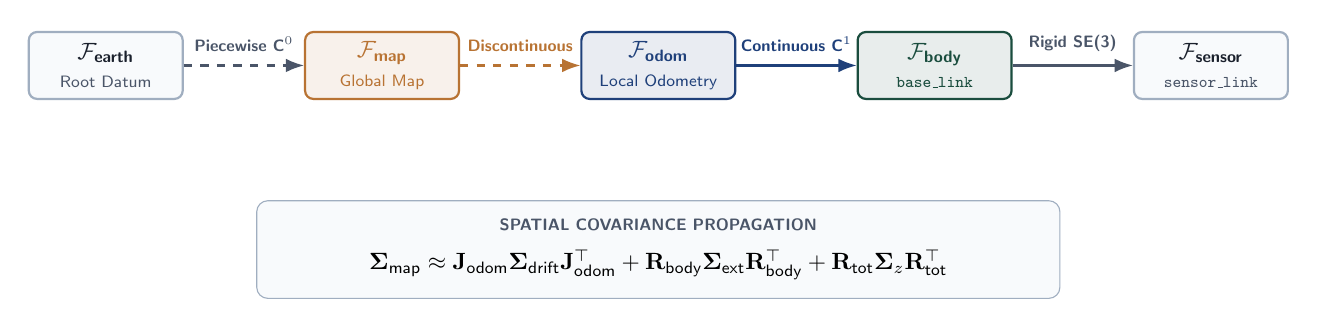
\begin{tikzpicture}[
    scale=0.85, transform shape,
    >=Latex,
    node distance=1.8cm,
    framebox/.style={
        rectangle,
        rounded corners=3pt,
        draw,
        thick,
        minimum width=2.3cm,
        minimum height=1.0cm,
        align=center,
        font=\sffamily
    },
    earth/.style={framebox, draw=paleink, fill=cardbg, text=ink},
    map/.style={framebox, draw=ethbronze, fill=ethbronze!10, text=ethbronze},
    odom/.style={framebox, draw=ethdarkblue, fill=ethdarkblue!10, text=ethdarkblue},
    body/.style={framebox, draw=emeraldpine, fill=emeraldpine!10, text=emeraldpine},
    sensor/.style={framebox, draw=paleink, fill=cardbg, text=ink},
    edge tag/.style={
        above,
        font=\sffamily\scriptsize\bfseries,
        align=center,
        yshift=2pt
    }
]

% Nodes
\node[earth]  (earth)  {\textbf{$\mathcal{F}_{\text{earth}}$}\\ \scriptsize\textcolor{softink}{Root Datum}};
\node[map]    (map)    [right=of earth] {\textbf{$\mathcal{F}_{\text{map}}$}\\ \scriptsize\textcolor{ethbronze}{Global Map}};
\node[odom]   (odom)   [right=of map]   {\textbf{$\mathcal{F}_{\text{odom}}$}\\ \scriptsize\textcolor{ethdarkblue}{Local Odometry}};
\node[body]   (body)   [right=of odom]  {\textbf{$\mathcal{F}_{\text{body}}$}\\ \scriptsize\textcolor{emeraldpine}{\texttt{base\_link}}};
\node[sensor] (sensor) [right=of body]  {\textbf{$\mathcal{F}_{\text{sensor}}$}\\ \scriptsize\textcolor{softink}{\texttt{sensor\_link}}};

% Edges
\draw[->, softink, thick, dashed] (earth) -- node[edge tag, text=softink] {Piecewise C$^0$} (map);
\draw[->, ethbronze, thick, dashed] (map) -- node[edge tag, text=ethbronze] {Discontinuous} (odom);
\draw[->, ethdarkblue, thick] (odom) -- node[edge tag, text=ethdarkblue] {Continuous C$^1$} (body);
\draw[->, softink, thick] (body) -- node[edge tag, text=softink] {Rigid SE(3)} (sensor);

% Bottom card
\node[
    rectangle, 
    rounded corners=4pt, 
    draw=paleink, 
    fill=cardbg, 
    minimum width=12cm, 
    inner sep=8pt,
    align=center,
    below=1.5cm of odom
] (cov) {
    \textbf{\scriptsize\color{softink} SPATIAL COVARIANCE PROPAGATION} \\[1ex]
    $\boldsymbol{\Sigma}_{\text{map}} \approx \mathbf{J}_{\text{odom}} \boldsymbol{\Sigma}_{\text{drift}} \mathbf{J}_{\text{odom}}^\top + \mathbf{R}_{\text{body}} \boldsymbol{\Sigma}_{\text{ext}} \mathbf{R}_{\text{body}}^\top + \mathbf{R}_{\text{tot}} \boldsymbol{\Sigma}_z \mathbf{R}_{\text{tot}}^\top$
};

\end{tikzpicture}
\end{document}
